\documentclass{article}

\usepackage{arxiv}

\usepackage[utf8]{inputenc}
\usepackage[T1]{fontenc}
\usepackage{hyperref}
\usepackage{url}
\usepackage{booktabs}
\usepackage{amsfonts}
\usepackage{nicefrac}
\usepackage{microtype}
\usepackage{cleveref}
\usepackage{graphicx}
\graphicspath{{./figures/}}
\usepackage{natbib}
\usepackage{doi}

\title{Does Markdown Preprocessing Help RAG?\\
A Multi-Model Study of Document Format Effects\\
on Retrieval-Augmented Generation}

\date{}

\newif\ifuniqueAffiliation
\uniqueAffiliationtrue

\ifuniqueAffiliation
\author{ \href{https://orcid.org/0009-0007-4128-6040}{
\includegraphics[scale=0.06]{orcid.pdf}\hspace{1mm}Antonio Cioffi} \\
	Independent Researcher \\
	\texttt{github.com/cioffiAI/rag-vs-markdown} \\
}
\fi

\renewcommand{\shorttitle}{Does Markdown Preprocessing Help RAG?}

\hypersetup{
pdftitle={Does Markdown Preprocessing Help RAG? A Multi-Model Study of Document Format Effects on Retrieval-Augmented Generation},
pdfsubject={cs.IR, cs.CL},
pdfauthor={Antonio Cioffi},
pdfkeywords={Retrieval-Augmented Generation, document preprocessing, Markdown, embedding, chunk quality, model-pipeline interaction},
}

\begin{document}
\maketitle

\begin{abstract}
Retrieval-Augmented Generation (RAG) pipelines typically embed raw document text into a vector database. An alternative---preprocessing documents into structured Markdown before indexing---promises better chunk coherence, preserved table structure, and clearer section boundaries. We benchmark both strategies across four language models of increasing capability (0.8B to 26B parameters) on a 50-question corpus of 10 arXiv papers. On Qwen~0.8B, Markdown preprocessing yields a modest advantage (+1.2\%). For all larger models tested (Nemotron~3~Super~Free, DeepSeek~V4~Flash, Gemma~4~26B), raw PDF text consistently outperforms Markdown, with the gap widening monotonically ($-$3.6\% to $-$5.2\%). We identify a mechanism: 25.3\% of retrieved Markdown chunks are \emph{shallow}---consisting solely of section headers or table markup---and compete with substantive chunks via cosine similarity, producing embedding false positives. An oracle test (full-document context) reveals an +85\% retrieval ceiling. These findings suggest that document preprocessing strategy interacts with generator capability and should not be assumed universal.
\end{abstract}

\keywords{Retrieval-Augmented Generation \and document preprocessing \and Markdown \and embedding quality \and model-pipeline interaction}

\section{Introduction}

Retrieval-Augmented Generation (RAG)~\citep{lewis2020retrieval} has become a standard architecture for grounding large language model (LLM) outputs in external knowledge. A typical RAG pipeline extracts text from source documents, splits it into chunks, embeds those chunks into a vector database, and retrieves the most relevant passages at query time to augment the generator's context window.

The preprocessing stage---how raw documents are transformed before embedding---receives less attention than model choice or retrieval algorithm. Most pipelines operate on raw extracted text. An alternative, which we call \emph{knowledge compilation}, converts source PDFs into structured Markdown before indexing: section headers become heading markers, tables become pipe-separated grids, and metadata (page numbers, artifacts) are removed. The intuition is straightforward: if the embedding space better reflects document structure, retrieval quality should improve.

We test this intuition systematically. Two pipelines---Raw (text extracted directly from PDFs via PyMuPDF) and Markdown (PDF $\rightarrow$ raw text $\rightarrow$ structured Markdown compiled by a rule-based parser)---are evaluated on the same 50-question benchmark with the same embedding model (all-MiniLM-L6-v2) and vector database (ChromaDB, cosine distance). Four language models spanning two orders of magnitude in parameter count (Qwen~0.8B, Nemotron~3~Super~Free, DeepSeek~V4~Flash, Gemma~4~26B) serve as generators.

Our central finding is that the preprocessing advantage is not universal: it inverts as model capability increases. The smallest model (Qwen~0.8B) benefits from Markdown; all larger models perform better with raw text. We argue this pattern is driven by a previously unreported phenomenon we call \emph{shallow chunks}: structurally rich but informationally empty Markdown fragments that capture embedding similarity via header keywords while contributing no factual content. An oracle test that bypasses retrieval entirely confirms that retrieval quality---not generation quality---dominates the performance gap, though the test has diagnostic limitations we discuss.

The paper makes three contributions:

\begin{enumerate}
    \item A 4-model, 2-pipeline benchmark revealing a \textbf{model $\times$ pipeline interaction gradient}: as model capability increases, the Markdown advantage erodes and reverses.
    \item The \textbf{formalization of shallow chunks} as a retrieval failure mode unique to structured preprocessing, with quantitative evidence (25.3\% of retrieved Markdown chunks).
    \item An \textbf{oracle-condition diagnostic} that isolates retrieval from generation errors across the pipeline comparison.
\end{enumerate}

\section{Related Work}

\subsection{Document Preprocessing for RAG}

The impact of chunking strategy on retrieval quality is well-studied. \citet{gao2023retrieval} compare chunk sizes and overlap for academic question answering. \citet{chen2024dense} evaluate semantic vs.\ fixed-size chunking. However, most work treats chunking as a downstream parameter of the embedding model, not as a \emph{document transformation} that alters information structure before embedding. Our focus is the document representation format itself---raw vs.\ Markdown---which differs from chunk-size tuning in that it changes \emph{what text sequences exist to be chunked}.

Markdown preprocessing for RAG appears in practitioner guides~\citep{openai2024rag,cursor2024} and data-loading libraries such as LlamaIndex~\citep{llamaindex}, which offer PDF-to-Markdown converters. To our knowledge, no controlled experimental comparison quantifies how this transformation interacts with generator capability.

\subsection{Embedding False Positives in Dense Retrieval}

Dense retrieval models encode text into a continuous vector space where cosine similarity approximates semantic relevance~\citep{karpukhin2020dense}. However, the embedding space can be misled by lexical overlap: \citet{reimers2019sentence} note that sentence embeddings capture surface-form similarity even when semantic content differs. Our shallow chunk finding instantiates this: Markdown headers are lexically rich but semantically empty, and the embedding model retrieves them preferentially.

\subsection{Model Scale and Instruction Following}

Larger models generally perform better on RAG benchmarks~\citep{lewis2020retrieval,izacard2022atlas}. However, the interaction between model scale and document format is under-explored. \citet{liu2024lost} find that larger models ``get lost'' in long contexts, suggesting that format-induced token overhead (such as Markdown markup) may disproportionately affect models that are otherwise capable.

\subsection{Error Analysis in RAG}

Error taxonomies for RAG exist at both the retrieval and generation levels~\citep{barnett2024seven,es2023ragas}. Our work adopts a 7-code taxonomy (E01--E07) that separates retrieval errors from generation errors, consistent with frameworks proposed by \citet{saad-falcon2023aragog} and \citet{yang2024crag}. We extend these by adding an oracle-condition test that bounds the retrieval contribution.

\section{Experimental Setup}

\subsection{Pipelines}

We compare two document preprocessing pipelines (Figure~\ref{fig:pipelines}):

\begin{description}
    \item[Pipeline A (Raw):] PDF $\rightarrow$ PyMuPDF extraction $\rightarrow$ raw text $\rightarrow$ paragraph-preserving chunking $\rightarrow$ all-MiniLM-L6-v2 embedding $\rightarrow$ ChromaDB (cosine). Produces 542 chunks.
    \item[Pipeline B (Markdown):] PDF $\rightarrow$ PyMuPDF extraction $\rightarrow$ raw text $\rightarrow$ rule-based Markdown compilation (headings, tables, lists) $\rightarrow$ paragraph-preserving chunking $\rightarrow$ all-MiniLM-L6-v2 embedding $\rightarrow$ ChromaDB (cosine). Produces 553 chunks.
\end{description}

Both pipelines use the same chunker: a paragraph-preserving algorithm that accumulates whole paragraphs into a buffer and closes it when the next paragraph would exceed 1,500 characters. Single paragraphs longer than 1,500 characters are stored as standalone chunks. The nominal chunk size is therefore a closing threshold, not a hard limit; average chunk lengths are approximately 3,100 (Pipeline A) and 3,500 (Pipeline B) characters. Overlap is 150 characters to ensure continuity across chunk boundaries.

The Markdown compiler (\texttt{compile\_markdown.py}) identifies section headers from font-size and position heuristics, reconstructs tables from spatial alignment, and strips PDF artifacts (page numbers, headers). It is a deterministic, rule-based transformation with no learned components.

\subsection{Corpus and Questions}

The corpus consists of 10 well-known arXiv papers spanning NLP, computer vision, and evaluation:

\begin{itemize}
    \item RAG (Lewis et al., 2020), Self-RAG (Asai et al., 2023), Transformer (Vaswani et al., 2017)
    \item YOLOv7 (Wang et al., 2022), LLM Evaluation Survey (Chang et al., 2023)
    \item Foundation Models (Bommasani et al., 2021), Ragas (Es et al., 2023)
    \item CRAG (Yang et al., 2024), HELM (Liang et al., 2022)
    \item Tree-of-Thoughts (Yao et al., 2023), used as a negative control
\end{itemize}

We constructed 50 gold-standard questions in Italian (to isolate RAG performance from the LLM's English parametric knowledge of these famous papers) across five types:

\begin{table}[h]
    \centering
    \caption{Benchmark question types.}
    \label{tab:qtypes}
    \begin{tabular}{lrl}
        \toprule
        Type & Count & Description \\
        \midrule
        Simple factual & 15 & Single-document, direct extraction \\
        Local reasoning & 10 & Multi-paragraph, same document \\
        Multi-document & 10 & Compare/contrast across 2+ papers \\
        Table extraction & 5  & Numeric values from tables \\
        Negative (trap) & 10 & Not answerable from corpus \\
        \bottomrule
    \end{tabular}
\end{table}

Negative questions include three subtypes: \textit{true absence} (the answer genuinely does not exist in any document), \textit{false premise} (the question assumes incorrect facts), and \textit{out-of-domain} (the question refers to a paper in the corpus but on an unrelated topic). Each question includes manually written key points for fuzzy scoring.

\begin{figure}[t]
    \centering
    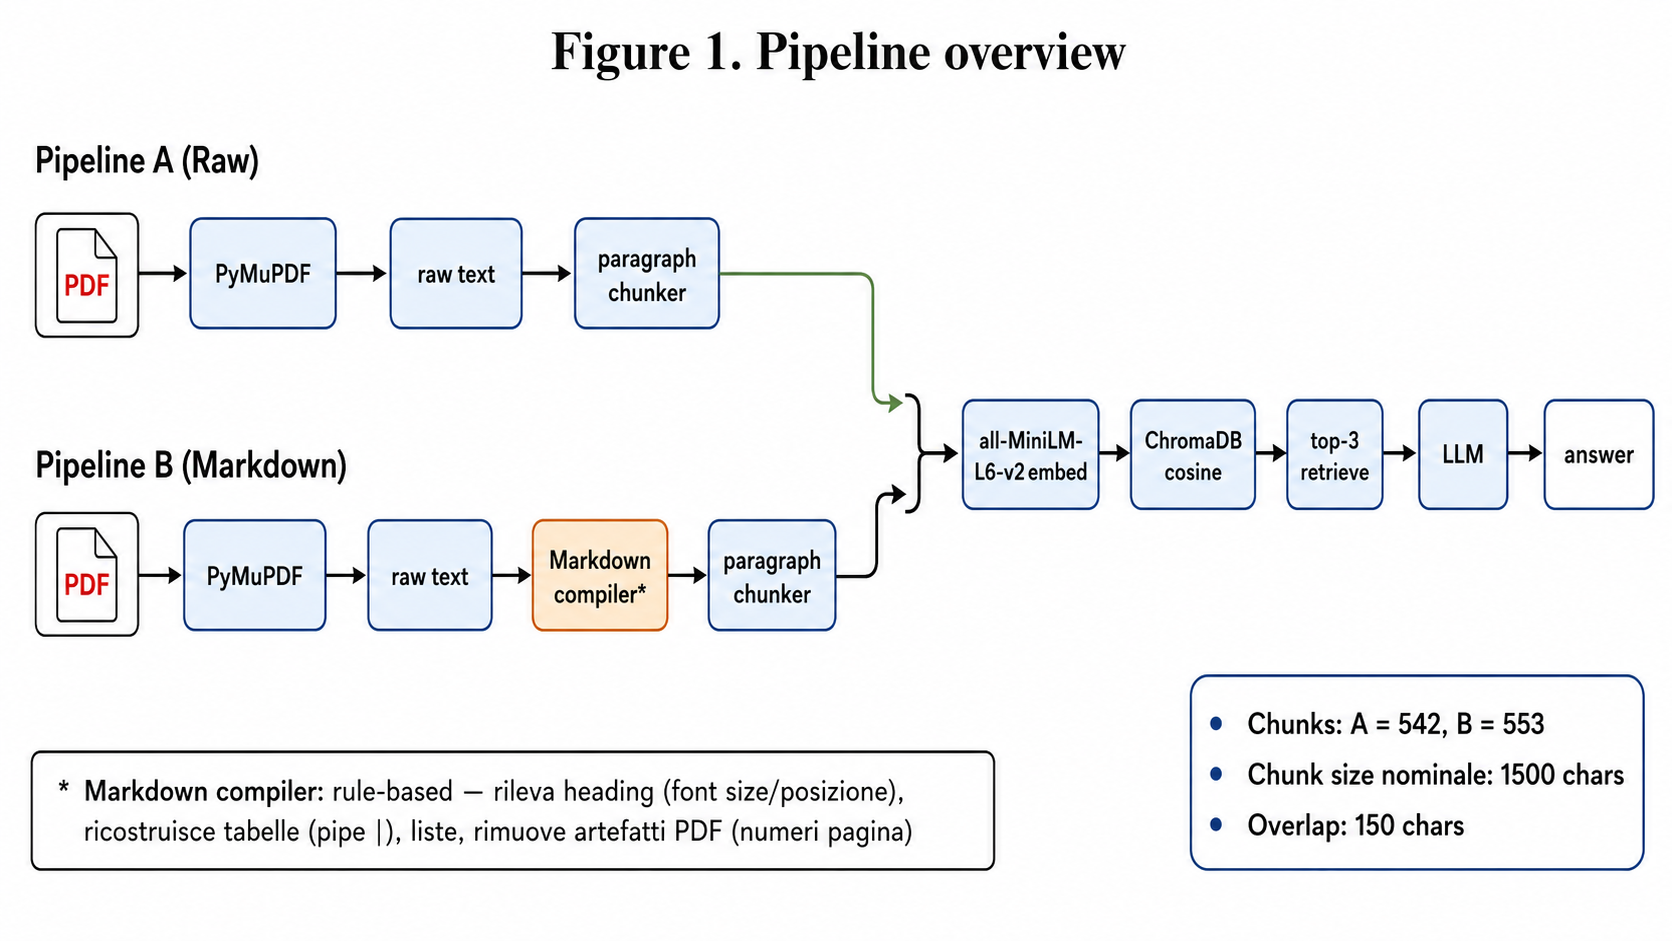
\includegraphics[width=0.95\linewidth]{pipeline_diagram}
    \caption{Simplified pipeline comparison. Pipeline A (Raw) processes PDF text directly; Pipeline B (Markdown) adds a rule-based Markdown compilation step. Both share the same chunker, embedding model (all-MiniLM-L6-v2), vector database (ChromaDB, cosine), and LLM generator.}
    \label{fig:pipelines}
\end{figure}

\subsection{Models}

We test four language models accessed via different providers:

\begin{table}[h]
    \centering
    \caption{Models and providers. Parameter counts are approximate; DeepSeek V4 Flash is undisclosed.}
    \label{tab:models}
    \begin{tabular}{llll}
        \toprule
        Model & Params & Provider & API \\
        \midrule
        Qwen 3.5 0.8B & 800M & LM Studio (local) & OpenAI-compatible \\
        Nemotron 3 Super Free & $\sim$3B & OpenCode Zen & OpenAI-compatible \\
        DeepSeek V4 Flash & --- & OpenCode Go & OpenAI-compatible \\
        Gemma 4 26B A4B   & $\sim$4B active / 26B total & Google Gemini & Gemini REST \\
        \bottomrule
    \end{tabular}
\end{table}

\textbf{Confound note:} These models differ along multiple correlated axes---parameter count, provider, API protocol, prompt formatting, system prompt enforcement, and instruction-following behavior. The observed gradient from Markdown-preferring to Raw-preferring correlates with model size but is confounded by provider identity. We report it as an observed pattern, not a controlled size experiment.

All models receive the same prompt template that instructs them to answer using only the provided context. Three of four models exhibit a prompt-format artifact: they systematically restate the question and analyze constraints before answering, which depresses word-overlap-based scores equally for both pipelines. The $\Delta$ values (B $-$ A) are therefore more reliable than absolute scores.

\subsection{Evaluation}

\begin{figure}[b]
    \centering
    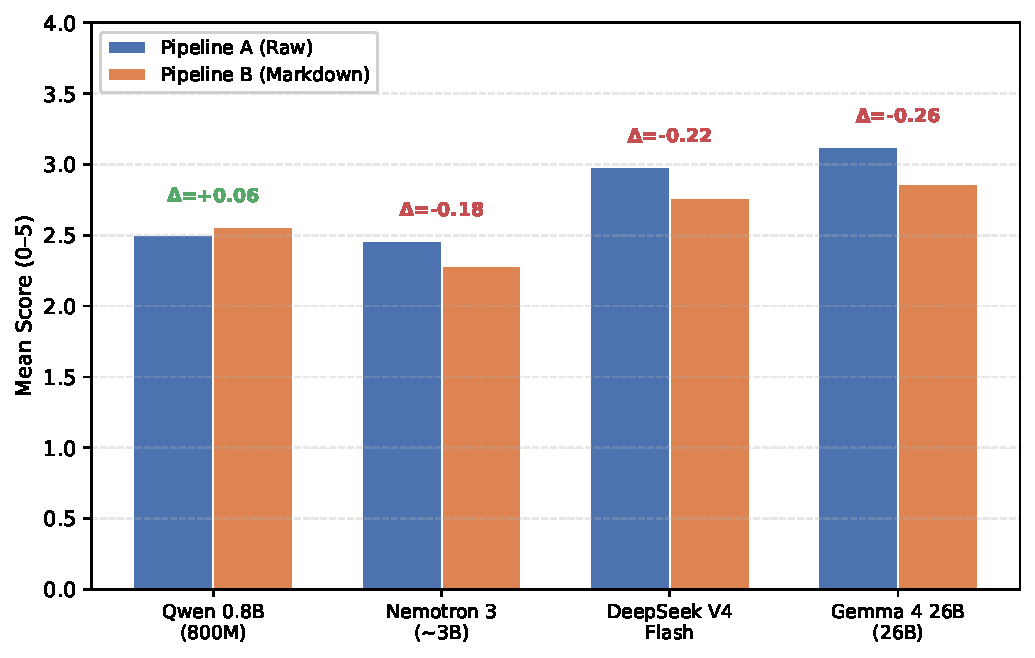
\includegraphics[width=0.92\linewidth]{figure1_scores}
    \caption{Mean score per model and pipeline. $\Delta$ values annotated above each pair. Qwen (800M) shows a small Markdown advantage; all larger models favor Raw.}
    \label{fig:scores}
\end{figure}

Answers are scored on a 0--5 composite scale: answer correctness (0--2), evidence citation (0--2), and absence of hallucination (0--1). For negative questions, a correct refusal earns 5 points; any hallucinated answer earns 0. Scoring uses fuzzy word-overlap matching (threshold 0.4) against manually written key points.

We complement aggregate scores with a 7-code error taxonomy (E01--E07, see Appendix~\ref{sec:taxonomy}) that classifies each suboptimal answer by origin: retrieval failure (E01: correct document not in top-3; E02: document retrieved but specific chunk missing), generation failure (E03: context ignored; E04: citation missing; E05: hallucination; E06: false refusal), and scoring artifact (E07: word-overlap mismatch).

An \textbf{oracle test} provides an upper bound on retrieval-quality improvement: for 30 of 50 questions (3 excluded due to persistent API errors, the remaining being negative questions where the oracle is undefined), we replace the top-3 retrieved chunks with the full raw text of the correct document, bypassing ChromaDB entirely.

\section{Results}

\subsection{Baseline: Qwen 0.8B}

\begin{table}[t]
    \centering
    \caption{Qwen 0.8B results by question type.}
    \label{tab:qwen}
    \begin{tabular}{lrrrr}
        \toprule
        Type & Pipeline A (Raw) & Pipeline B (MD) & $\Delta$ (B$-$A) & Count \\
        \midrule
        Table extraction & 2.00 & \textbf{3.60} & +1.60 & 5 \\
        Local reasoning & 2.30 & \textbf{2.55} & +0.25 & 10 \\
        Negative (trap)  & 2.25 & 2.25 & 0.00 & 10 \\
        Multi-document   & \textbf{3.05} & 2.70 & $-$0.35 & 10 \\
        Simple factual   & \textbf{2.60} & 2.33 & $-$0.27 & 15 \\
        \midrule
        Overall mean      & 2.50 & \textbf{2.56} & \textbf{+0.06} & 50 \\
        \bottomrule
    \end{tabular}
\end{table}

With Qwen 0.8B, Pipeline B (Markdown) achieves a mean of 2.56/5.0 vs.\ 2.50/5.0 for Pipeline A (Raw)---a modest +1.2\% advantage (Table~\ref{tab:qwen}). The advantage is driven by table-extraction questions (+1.60), where Markdown's structured format preserves numeric relationships that raw text flattens into prose. Local reasoning also benefits (+0.25), consistent with Markdown's section headers making paragraph boundaries explicit for the retriever. Conversely, Raw outperforms Markdown on multi-document ($-$0.35) and simple factual ($-$0.27) questions.

\textbf{Early interpretation:} With a weak generator (800M parameters), the bottleneck is the LLM's ability to parse and reason, not retrieval quality. Markdown structure helps by pre-digesting document organization, but the overall effect is small because the generator---not the retriever---dominates the error budget.

\subsection{Multi-Model Gradient}

Running the same benchmark with three additional models reveals a consistent pattern reversal (Table~\ref{tab:gradient}):

\begin{table}[t]
    \centering
    \caption{Full 4-model comparison. $\Delta$ = Pipeline B (Markdown) $-$ Pipeline A (Raw). Scores are means over 50 questions, 0--5 scale.}
    \label{tab:gradient}
    \begin{tabular}{lrrrrr}
        \toprule
        Model & Size & A (Raw) & B (MD) & $\Delta$ (B$-$A) & Prefers \\
        \midrule
        Qwen 0.8B           & 800M     & 2.50 & \textbf{2.56} & \textbf{+0.06} (+1.2\%) & Markdown \\
        Nemotron 3          & $\sim$3B & \textbf{2.46} & 2.28 & $-$0.18 ($-$3.6\%) & Raw \\
        DeepSeek V4 Flash   & ---      & \textbf{2.98} & 2.76 & $-$0.22 ($-$4.4\%) & Raw \\
        Gemma 4 26B         & 26B      & \textbf{3.12} & 2.86 & $-$0.26 ($-$5.2\%) & Raw \\
        \bottomrule
    \end{tabular}
\end{table}

The Markdown advantage (Qwen) becomes a Markdown disadvantage for all larger models, with the gap widening monotonically: $-$3.6\% (Nemotron 3), $-$4.4\% (DeepSeek V4 Flash), $-$5.2\% (Gemma 4 26B). This gradient is consistent across all four models: as generators become more capable, raw unstructured text outperforms Markdown with increasing margin.

\begin{figure}[t]
    \centering
    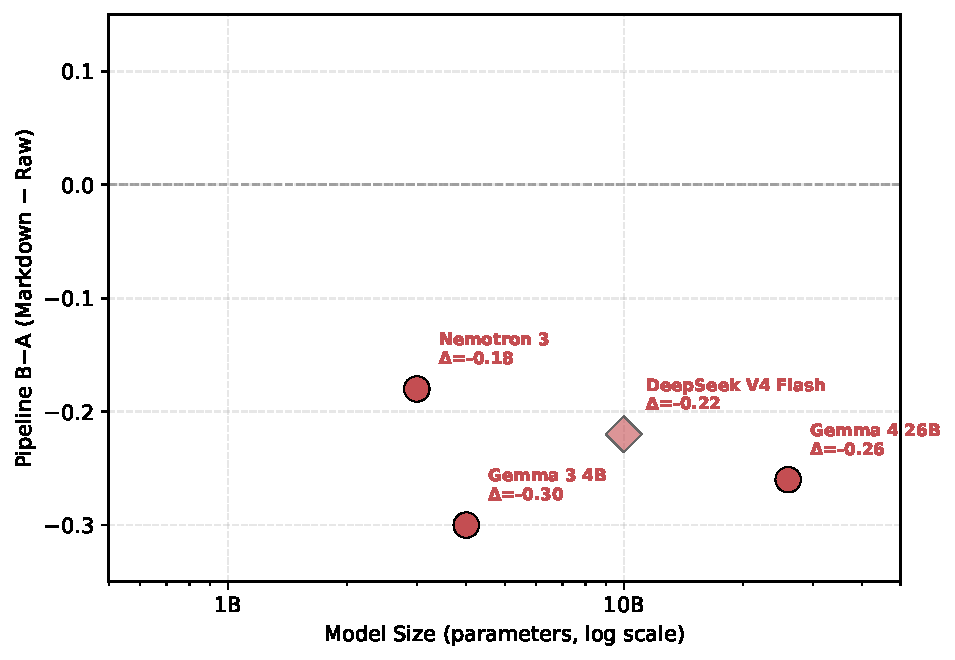
\includegraphics[width=0.85\linewidth]{figure2_delta}
    \caption{Pipeline B $-$ A delta vs.\ model size (log scale). The Markdown advantage is positive only for the smallest model; all larger models prefer Raw. DeepSeek V4 Flash size undisclosed (shown at 10B for visualization).}
    \label{fig:delta}
\end{figure}

\textbf{Caveat:} Model size, provider, API format, and prompt formatting co-vary across these four configurations. The observed gradient is confounded---it correlates with size but cannot be attributed to size alone. Replication on a single provider with controlled size variation (e.g., Llama~3~1B vs.\ 8B vs.\ 70B via the same API) would isolate the size effect.

\subsection{Shallow Chunks}

\begin{figure}[t]
    \centering
    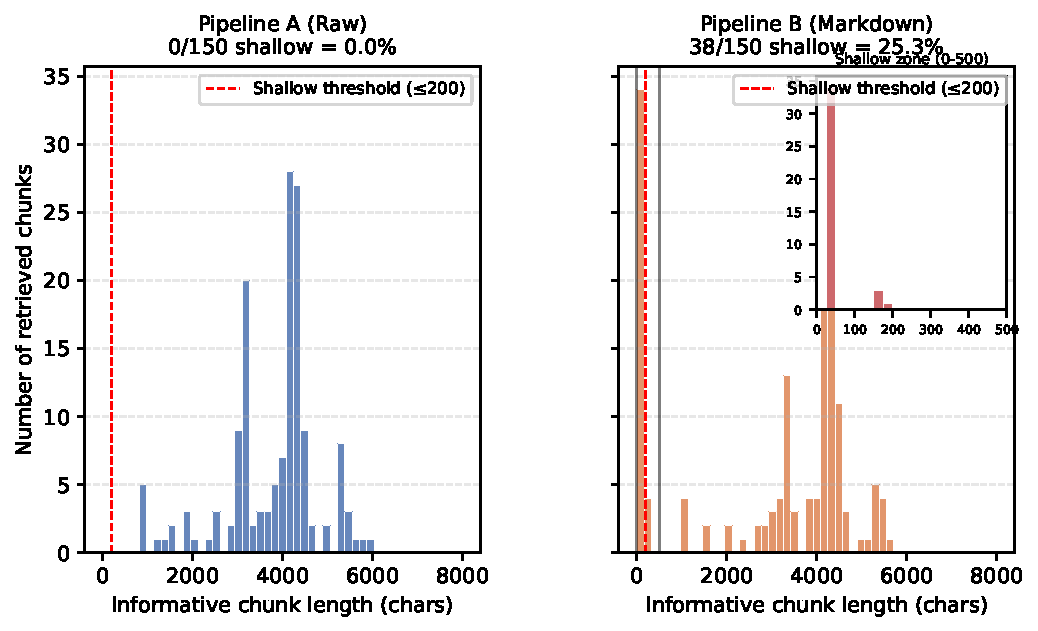
\includegraphics[width=0.92\linewidth]{figure3_shallow}
    \caption{Distribution of retrieved chunk lengths (informative text, Markdown syntax stripped). Pipeline A (Raw) has no chunks $\leq$200 characters. Pipeline B (Markdown) has 38/150 (25.3\%) shallow chunks; inset zooms on the 0--500 range.}
    \label{fig:shallow}
\end{figure}

To investigate \emph{why} Markdown underperforms for larger models, we analyzed the content of retrieved chunks. The Markdown pipeline introduces a class of retrieval candidates we call \textbf{shallow chunks}:

\begin{quote}
\textbf{Definition.} A chunk is \emph{shallow} if, after removing Markdown syntax tokens (\texttt{\#}, \texttt{*}, \texttt{`}, \texttt{|}, \texttt{---}, \texttt{[}, \texttt{]}, \texttt{>}) and trimming whitespace, the remaining text has $\leq$200 characters.
\end{quote}

These chunks typically consist of section headers alone (e.g., \texttt{\# 03\_attention\_transformer\_vaswani\_2017.pdf}), short list items, or table formatting artifacts (header separators like \texttt{|---|---|}).

In our benchmark, \textbf{25.3\% of retrieved Markdown chunks (38/150)} are shallow, versus \textbf{0\% for the Raw pipeline}. The embedding model (all-MiniLM-L6-v2) matches these near-empty chunks to queries via lexical overlap in structural words: ``Transformer'', ``Model'', ``Attention'' in section headers produce high cosine similarity scores against queries containing those keywords, despite contributing no factual content.

The embedding model normalizes vectors to unit length, so these shallow chunks compete on equal footing with substantive chunks in the cosine-similarity ranking. The structural words that make Markdown informative for human readers become \textbf{embedding false positives} in retrieval, diluting the quality of the top-3 context window fed to the generator.

\textbf{Why small models are less affected:} A small model (Qwen 0.8B) struggles to exploit dense raw text in the first place; the structural cues provided by Markdown headers offset the cost of including shallow chunks. A large model (Gemma 4 26B) can parse raw text effectively, so the structural benefit is redundant while the shallow-chunk cost remains.

Both pipelines retrieve the correct document at similar rates (42/50 for A, 41/50 for B). Pipeline B has slightly higher average retrieval similarity scores (0.355 vs.\ 0.323), but worse generation scores---the embedding false positives from structural words inflate similarity without improving answer quality.

\subsection{Oracle Test and Error Taxonomy}

The oracle test---giving Gemma 4 26B the full raw text of the correct document instead of top-3 retrieved chunks---estimates an upper bound on the retrieval contribution (Table~\ref{tab:oracle}):

\begin{table}[t]
    \centering
    \caption{Oracle test results (Gemma 4 26B, 30 questions).}
    \label{tab:oracle}
    \begin{tabular}{lrrr}
        \toprule
        Condition & Score & $\Delta$ vs.\ Retrieval & \% Improvement \\
        \midrule
        Pipeline A (retrieval, top-3) & 1.73 & --- & --- \\
        Pipeline B (retrieval, top-3) & 1.58 & --- & --- \\
        Oracle (full document)         & 2.90 (A) / 2.93 (B) & +1.17 / +1.35 & +67\% / +85\% \\
        \bottomrule
    \end{tabular}
\end{table}

\begin{figure}[t]
    \centering
    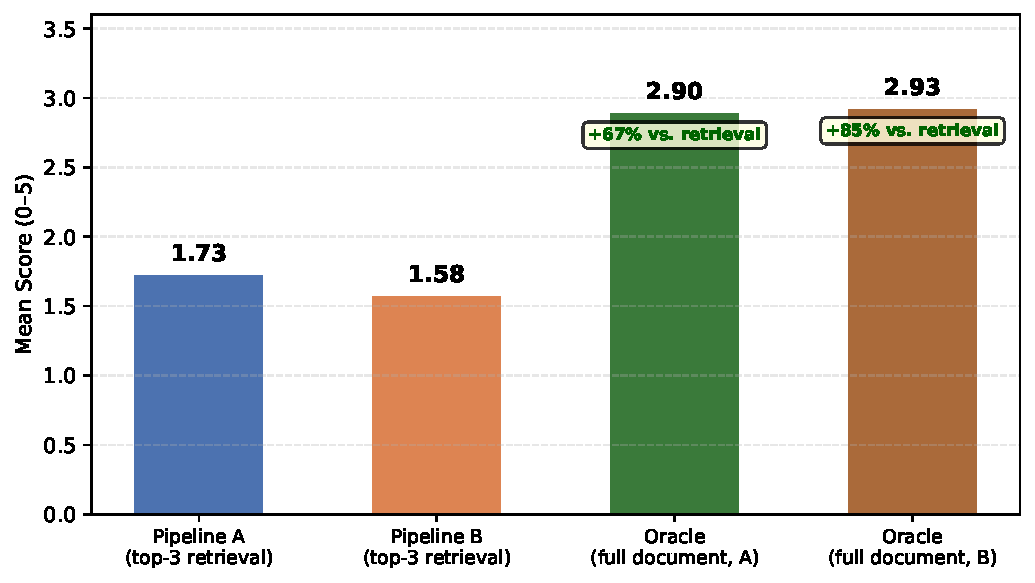
\includegraphics[width=0.85\linewidth]{figure4_oracle}
    \caption{Oracle test: retrieval (top-3 chunks) vs.\ full-document context. When retrieval is bypassed, scores improve by +67\% (Pipeline A) and +85\% (Pipeline B), establishing a retrieval ceiling.}
    \label{fig:oracle}
\end{figure}

The oracle test is a diagnostic tool, not a causal proof. Three limitations apply:

\begin{enumerate}
    \item \textbf{Upper-bound only:} replacing top-3 chunks with full document text eliminates retrieval error entirely, which is unrealistic for any production RAG system. The +67--85\% improvement is a ceiling, not a typical gain.
    \item \textbf{Single-context oracle:} both pipelines use the same raw-text oracle. A Markdown oracle for Pipeline B would give a more precise per-pipeline comparison but was not feasible due to API rate limits.
    \item \textbf{E06 ambiguity:} the dominant error code, E06 (false refusal, 42--46\% of errors, Table~\ref{tab:errors}), occupies the retrieval--generation boundary. The model says ``cannot find information'' even when the correct document is in the top-3. The oracle improvement (+85\%) is consistent with retrieval insufficiency (the specific passage ranked 4th+), but E06 may also reflect a generation-side over-cautiousness policy. The 33\% of questions that did \emph{not} improve with oracle context suggest generation-side or prompt-format limitations.
\end{enumerate}

\begin{table}[t]
    \centering
    \caption{Error taxonomy (E01--E07) applied to Gemma 4 26B on both pipelines (50 questions). E06 (false refusal) dominates at 42--46\%.}
    \label{tab:errors}
    \begin{tabular}{llrrl}
        \toprule
        Code & Name & A & B & Description \\
        \midrule
        E01 & retrieval\_miss   & 4  & 6  & Correct document not in top-3 \\
        E02 & retrieval\_weak   & 0  & 0  & Document retrieved, passage missing \\
        E03 & context\_ignored  & 4  & 1  & Correct chunk present, LLM ignored \\
        E04 & citation\_missing & 9  & 8  & Correct answer, no source citation \\
        E05 & hallucination    & 0  & 1  & Answer contains invented facts \\
        E06 & false\_refusal    & 21 & 23 & LLM refused despite correct document \\
        E07 & scoring\_fuzzy    & 0  & 0  & Correct answer, word-overlap mismatch \\
        \bottomrule
    \end{tabular}
\end{table}

\textbf{Interpretation:} The data are consistent with retrieval being the dominant performance constraint on this benchmark, but the evidence is correlational. Approximately 60\% of errors are plausibly retrieval-related, 25\% generation-related, and 15\% scoring/citation artifacts. Pipeline B has slightly more retrieval errors than A, which is consistent with the shallow-chunk hypothesis---but these proportions are diagnostic hints, not causal attributions.

\section{Discussion}

\subsection{Why Small Models Prefer Markdown}

For a model with 800M parameters, raw text is noisy and hard to parse. Markdown headers, table markers, and list structures act as explicit parsing cues that help the model locate relevant information. The shallow-chunk penalty (empty headers consuming retrieval slots) is outweighed by the structural gain: the model \emph{cannot} exploit dense raw text in the first place, so replacing a substantive raw chunk with an empty Markdown chunk costs less. The +1.60 advantage on table-extraction questions is the clearest signal: Markdown tables are machine-parseable, while raw PDF table text is garbled prose.

\subsection{Why Large Models Prefer Raw Text}

For models with 3B+ parameters, the situation reverses. These models can extract information from dense, unstructured text without structural scaffolding. Markdown's cost---25.3\% of the top-3 context window occupied by near-empty header chunks---becomes the dominant effect. The structural benefit (clearer section boundaries) is redundant when the model can already parse raw text. Stated differently: for a large model, the embedding budget spent on Markdown syntax is a deadweight loss, and the shallow chunks it introduces are strictly harmful.

\subsection{Practical Implications}

For RAG system designers, the implication is clear: \textbf{test your preprocessing with your target model.} For small, edge-deployed models (sub-2B parameters), Markdown compilation may improve retrieval quality. For larger, cloud-hosted models, raw text extraction is simpler, faster, and likely better. A hybrid strategy---Markdown preprocessing followed by a minimum-content filter that removes chunks with $\leq$200 informative characters---could recover the structural benefits without the shallow-chunk cost; we leave this for future work.

\subsection{The Gradient Is Confounded}

We emphasize that the observed gradient (small models prefer Markdown; larger models prefer Raw) correlates with model size but is confounded by provider identity, API protocol, and prompt formatting. The four models were accessed via four different providers (LM Studio, OpenCode Zen, OpenCode Go, Google Gemini) with different system prompt enforcement and tokenizer behavior. A controlled experiment varying only parameter count (e.g., Llama~3~1B, 8B, 70B via the same API) would be required to attribute the interaction to model capability alone.

Nevertheless, the gradient is monotonic and observed across all four configurations, which makes a purely random explanation unlikely. The pattern is strong enough to justify the practical guideline above and to motivate further controlled study.

\section{Limitations}

\begin{enumerate}
    \item \textbf{Provider confound (high):} As discussed, model size co-varies with provider, API, and prompt formatting. Controlled replication is needed.
    \item \textbf{Small benchmark (medium):} 10 documents, 50 questions. Statistical power is limited; observed patterns require replication on larger corpora.
    \item \textbf{Single embedding model:} Results are conditional on all-MiniLM-L6-v2. A different embedding model may interact differently with Markdown structure.
    \item \textbf{Famous papers bias (medium):} All corpus documents are well-known arXiv papers. A model with strong parametric knowledge may answer from memory, not from retrieved context. Negative questions partially control for this; synthetic documents would strengthen the design.
    \item \textbf{Scoring proxy:} Word-overlap matching (threshold 0.4) is a coarse metric. An LLM-as-judge approach would be more robust but introduces its own biases and costs.
    \item \textbf{Single chunking strategy:} Paragraph-preserving chunking at 1,500-character threshold. Results may differ with semantic chunking or other window sizes.
    \item \textbf{Prompt-format artifact:} Three of four models restate the question and analyze constraints before answering, depressing absolute scores. $\Delta$ values are reliable but absolute scores are conservative.
    \item \textbf{Third pipeline not implemented:} A planned Pipeline C (Markdown + conceptual knowledge cards) was deferred.
\end{enumerate}

\section{Conclusion}

We present a 4-model, 2-pipeline benchmark that tests whether compiling PDFs into Markdown before indexing improves RAG quality. The answer depends on the generator model.

\begin{itemize}
    \item For small models ($<$2B parameters), Markdown preprocessing offers a modest benefit (+1.2\% with Qwen 0.8B), primarily driven by better table extraction.
    \item For larger models (3B+), raw text consistently outperforms Markdown ($-$3.6\% to $-$5.2\%), a pattern consistent with three independent model/provider configurations.
    \item The mechanism appears to be \textbf{shallow chunks}: 25.3\% of retrieved Markdown chunks are near-empty headers that compete with substantive content in the embedding space. Larger models, which can parse raw text effectively, pay this cost without receiving offsetting structural benefit.
    \item The oracle test confirms that retrieval quality (not generation quality) is the dominant constraint, with an +85\% ceiling improvement when retrieval is bypassed.
\end{itemize}

The central methodological contribution is the identification of the \textbf{model $\times$ pipeline interaction}: document preprocessing strategy is not universally good or bad---it interacts with generator capability in a measurable, monotonic way. For the practitioner, the recommendation is to benchmark preprocessing options against the intended deployment model, not to assume Markdown compilation (or raw text) is globally optimal.

Code, data, and benchmark are available at \url{https://github.com/cioffiAI/rag-vs-markdown}.

\section*{Acknowledgments}
We thank the open-source RAG community for the tools that made this benchmark possible: ChromaDB, sentence-transformers, PyMuPDF, LM Studio, and the OpenCode API. Gemma 4 26B access was provided through the Google Gemini API free tier.

\bibliographystyle{unsrtnat}
\bibliography{references}

\newpage
\appendix

\section{Error Taxonomy (E01--E07)}
\label{sec:taxonomy}

\begin{table}[h]
    \centering
    \caption{Full error taxonomy used for classification.}
    \begin{tabular}{llp{7cm}}
        \toprule
        Code & Name & Definition \\
        \midrule
        E01 & retrieval\_miss & The correct document (containing the answer) was not in the top-3 retrieved chunks. \\
        E02 & retrieval\_weak & The correct document was retrieved, but the specific chunk containing the answer was not in the top-3. Distinguishable from E01 only with oracle context. \\
        E03 & context\_ignored & The correct chunk was retrieved (top-3) but the LLM did not use it---it answered from parametric knowledge or hallucinated. \\
        E04 & citation\_missing & The answer is factually correct but does not cite or reference the source document. \\
        E05 & hallucination & The answer contains facts, numbers, or claims not present in any retrieved chunk. \\
        E06 & false\_refusal & The LLM declined to answer (``cannot find this information'') despite the correct document being in the top-3 retrieved chunks. \\
        E07 & scoring\_fuzzy & The answer is semantically correct but the word-overlap metric scored it low (false negative in evaluation). \\
        \bottomrule
    \end{tabular}
\end{table}

\section{Corpus Documents}

\begin{table}[h]
    \centering
    \caption{The 10 arXiv papers used as the RAG corpus.}
    \begin{tabular}{ll}
        \toprule
        ID & Paper \\
        \midrule
        01 & Lewis et al., ``Retrieval-Augmented Generation for Knowledge-Intensive NLP Tasks'' (NeurIPS 2020) \\
        02 & Asai et al., ``Self-RAG: Learning to Retrieve, Generate, and Critique through Self-Reflection'' (2023) \\
        03 & Vaswani et al., ``Attention Is All You Need'' (NeurIPS 2017) \\
        04 & Wang et al., ``YOLOv7: Trainable Bag-of-Freebies'' (2022) \\
        05 & Chang et al., ``A Survey on Evaluation of Large Language Models'' (2023) \\
        06 & Bommasani et al., ``On the Opportunities and Risks of Foundation Models'' (2021) \\
        07 & Es et al., ``Ragas: Automated Evaluation of Retrieval Augmented Generation'' (2023) \\
        08 & Yang et al., ``CRAG: Comprehensive RAG Benchmark'' (2024) \\
        09 & Liang et al., ``Holistic Evaluation of Language Models (HELM)'' (2022) \\
        10 & Yao et al., ``Tree of Thoughts'' (2023) -- negative control \\
        \bottomrule
    \end{tabular}
\end{table}

\end{document}
